\documentclass[border=10pt]{standalone}
\usepackage[svgnames]{xcolor}
\usepackage{amsmath}
\usepackage{pgfplots}
\pgfplotsset{compat=newest}
\usepackage[sfdefault]{FiraSans}
\usepackage{FiraMono}
\renewcommand*\familydefault{\sfdefault}
\begin{document}
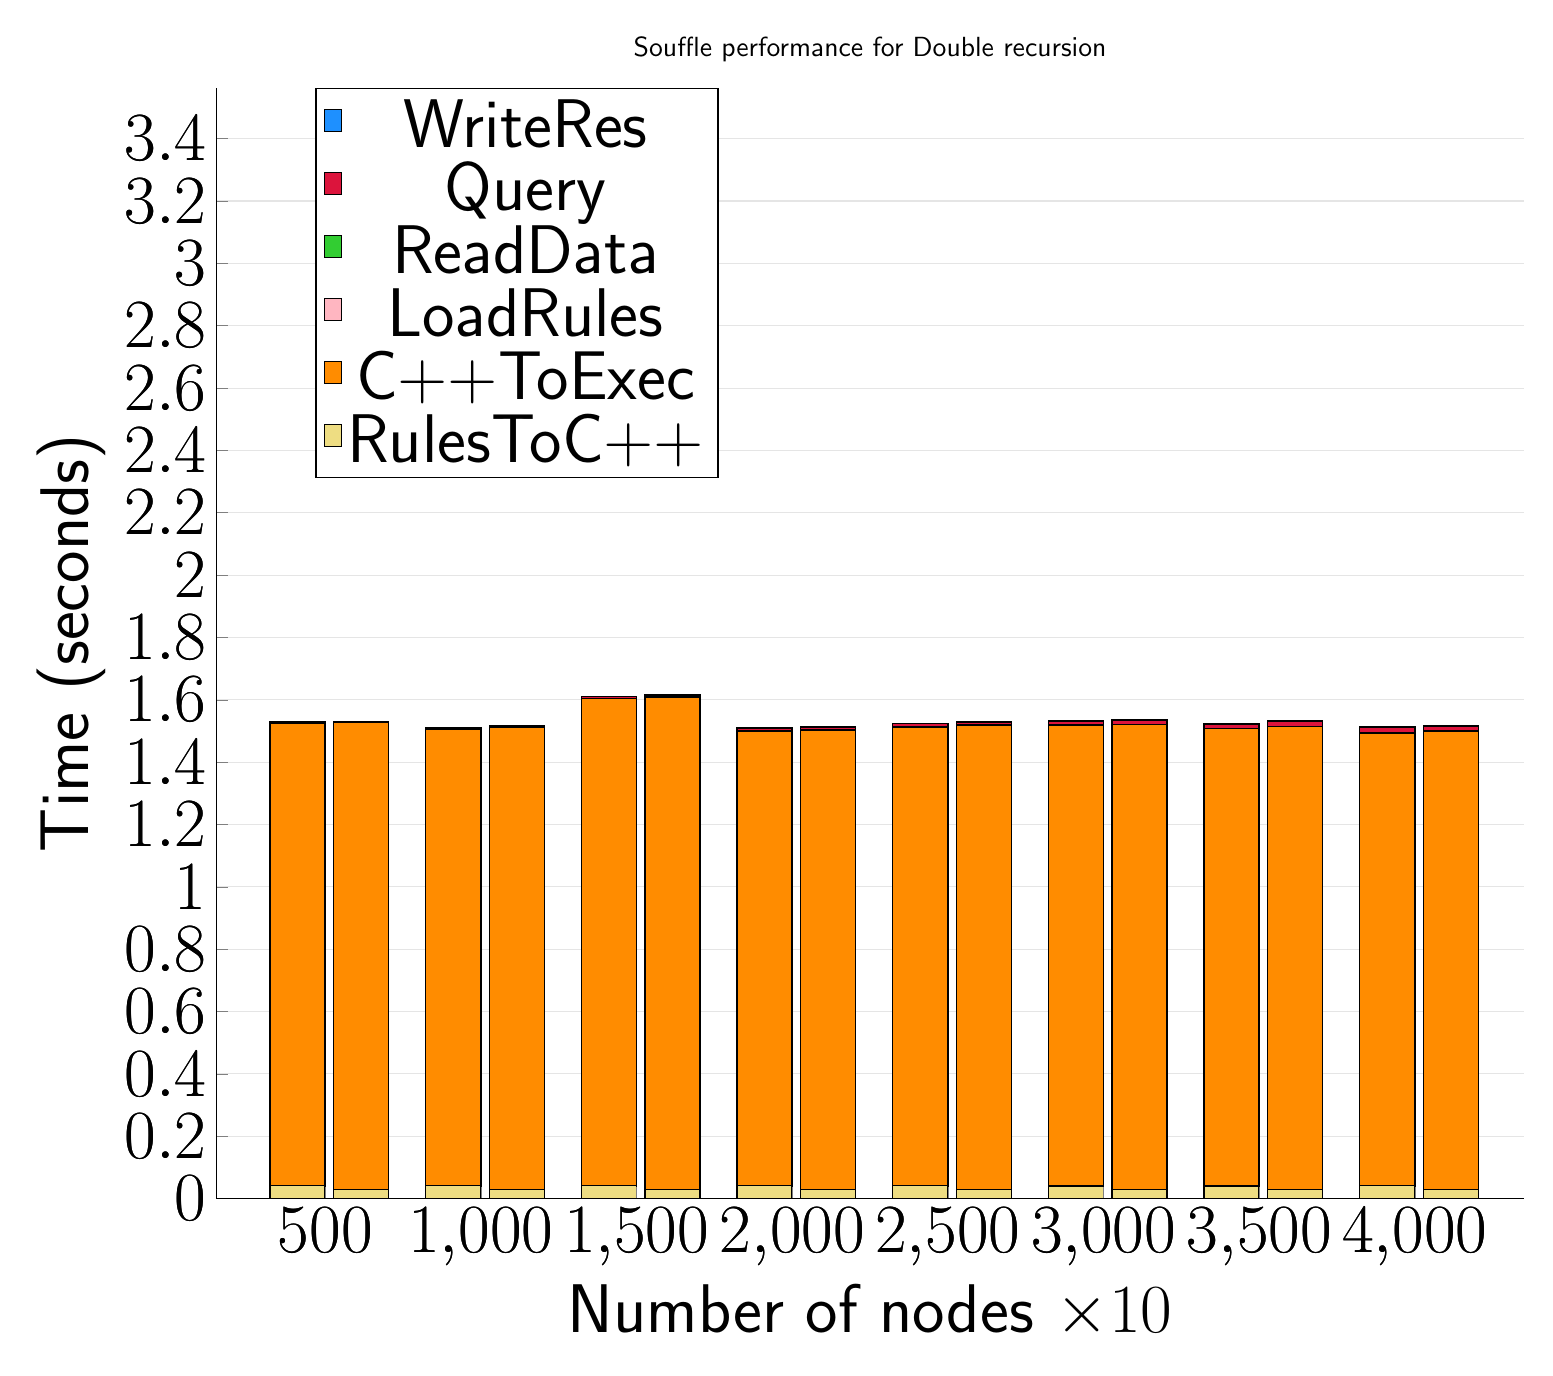
\begin{tikzpicture}
\begin{axis}[
   ybar stacked,
   title={Souffle performance for Double recursion},
   bar shift=-10pt,
   width=1.5\textwidth,
   bar width=0.7cm,
   ymajorgrids, tick align=inside,
   major grid style={draw=gray!20},
   xtick=data,
   ymin=0, ymax=3.562999987602234,
   axis x line*=bottom,
   axis y line*=left,
   enlarge x limits=0.1,
   legend style={
       at={(0.23, 1)},
       anchor=north,
       legend columns=1,
       font=\Huge,
   },
   ylabel={Time (seconds)},
   xlabel={Number of nodes $\times 10$},
   label style={font=\Huge},
   tick label style={font=\Huge},
]
\addlegendimage{fill=DodgerBlue, draw=black, line width=0.2pt}
\addlegendentry{WriteRes}
\addlegendimage{fill=Crimson, draw=black, line width=0.2pt}
\addlegendentry{Query}
\addlegendimage{fill=LimeGreen, draw=black, line width=0.2pt}
\addlegendentry{ReadData}
\addlegendimage{fill=LightPink, draw=black, line width=0.2pt}
\addlegendentry{LoadRules}
\addlegendimage{fill=DarkOrange, draw=black, line width=0.2pt}
\addlegendentry{C++ToExec}
\addlegendimage{fill=LightGoldenrod, draw=black, line width=0.2pt}
\addlegendentry{RulesToC++}
\addplot +[fill=LightGoldenrod, draw=black, line width=0.5pt] coordinates {
    (500, 0.04100003242492676)
    (1000, 0.04100005626678467)
    (1500, 0.040999960899353025)
    (2000, 0.04100003242492676)
    (2500, 0.04200000762939453)
    (3000, 0.039999985694885255)
    (3500, 0.04000003337860107)
    (4000, 0.04100003242492676)
};
\addplot +[fill=DarkOrange, draw=black, line width=0.5pt] coordinates {
    (500, 1.4850000143051147)
    (1000, 1.4629999637603759)
    (1500, 1.5629999876022338)
    (2000, 1.4589999675750733)
    (2500, 1.4700000047683717)
    (3000, 1.478000020980835)
    (3500, 1.4669999837875367)
    (4000, 1.452999973297119)
};
\addplot +[fill=LightPink, draw=black, line width=0.5pt] coordinates {
    (500, 0.0001079458)
    (1000, 0.00011205820000000002)
    (1500, 6.093349999999999e-05)
    (2000, 0.0001249248)
    (2500, 0.00010828340000000002)
    (3000, 9.605e-05)
    (3500, 0.00012309160000000002)
    (4000, 0.00011155839999999999)
};
\addplot +[fill=LimeGreen, draw=black, line width=0.5pt] coordinates {
    (500, 0.0003636582)
    (1000, 0.0004921043)
    (1500, 0.0004966294000000001)
    (2000, 0.0007159957)
    (2500, 0.0007854333999999999)
    (3000, 0.000861796)
    (3500, 0.0010365476999999999)
    (4000, 0.0011179731)
};
\addplot +[fill=Crimson, draw=black, line width=0.5pt] coordinates {
    (500, 0.002258926)
    (1000, 0.004555108)
    (1500, 0.005415949)
    (2000, 0.008811006)
    (2500, 0.010500812)
    (3000, 0.01228664)
    (3500, 0.014682980000000002)
    (4000, 0.01629974)
};
\addplot +[fill=DodgerBlue, draw=black, line width=0.5pt] coordinates {
    (500, 0.0006058871999999999)
    (1000, 0.0008787538999999999)
    (1500, 0.0008978546)
    (2000, 0.00127275)
    (2500, 0.001307919)
    (3000, 0.0013940950000000001)
    (3500, 0.00168938)
    (4000, 0.0018187040000000002)
};
\end{axis}
\begin{axis}[
   ybar stacked,
   bar shift=13pt,
   width=1.5\textwidth,
   bar width=0.7cm,
   ymajorgrids, tick align=inside,
   major grid style={draw=none},
   xtick=data,
   ymin=0, ymax=3.562999987602234,
   axis x line*=none,
   axis y line*=none,
   enlarge x limits=0.1,
   label style={font=\Huge},
   tick label style={font=\Huge},
]
\addplot +[fill=LightGoldenrod, draw=black, line width=0.5pt] coordinates {
    (500, 0.030000000000000006)
    (1000, 0.030000000000000006)
    (1500, 0.030000000000000006)
    (2000, 0.030000000000000006)
    (2500, 0.030000000000000006)
    (3000, 0.030000000000000006)
    (3500, 0.030000000000000006)
    (4000, 0.030000000000000006)
};
\addplot +[fill=DarkOrange, draw=black, line width=0.5pt] coordinates {
    (500, 1.498)
    (1000, 1.4820000000000002)
    (1500, 1.5790000000000002)
    (2000, 1.472)
    (2500, 1.488)
    (3000, 1.49)
    (3500, 1.4840000000000002)
    (4000, 1.469)
};
\addplot +[fill=LightPink, draw=black, line width=0.5pt] coordinates {
    (500, 0.00010729999999999999)
    (1000, 0.00011129999999999998)
    (1500, 6.03e-05)
    (2000, 0.0001238)
    (2500, 0.0001077)
    (3000, 9.57e-05)
    (3500, 0.0001226)
    (4000, 0.0001107)
};
\addplot +[fill=LimeGreen, draw=black, line width=0.5pt] coordinates {
    (500, 0.00036290000000000004)
    (1000, 0.0004902)
    (1500, 0.0004959)
    (2000, 0.000715)
    (2500, 0.0007844999999999999)
    (3000, 0.0008608999999999998)
    (3500, 0.0010358)
    (4000, 0.0011169)
};
\addplot +[fill=Crimson, draw=black, line width=0.5pt] coordinates {
    (500, 0.0022580000000000005)
    (1000, 0.0045523000000000004)
    (1500, 0.005413799999999999)
    (2000, 0.0088061)
    (2500, 0.0104908)
    (3000, 0.0122657)
    (3500, 0.0146638)
    (4000, 0.0162799)
};
\addplot +[fill=DodgerBlue, draw=black, line width=0.5pt] coordinates {
    (500, 0.0004535)
    (1000, 0.0006888)
    (1500, 0.000796)
    (2000, 0.0011281999999999998)
    (2500, 0.0012232999999999999)
    (3000, 0.0013644000000000002)
    (3500, 0.0016004000000000005)
    (4000, 0.0017353999999999998)
};
\end{axis}
\end{tikzpicture}

\end{document}
